\documentclass[10pt,twocolumn,letterpaper]{article}

\usepackage[pagenumbers]{cvpr}
\usepackage{graphicx}
\usepackage{amsmath}
\usepackage{amssymb}
\usepackage{booktabs}
\usepackage[utf8]{inputenc}
\usepackage{graphicx}
\usepackage{scalefnt}
\usepackage{textfit}
\usepackage{float}
\usepackage{cite}
\usepackage{stmaryrd}
\usepackage{bm}
\usepackage[linesnumbered,lined,boxed,ruled,commentsnumbered]{algorithm2e}
\usepackage{algorithmic}
\usepackage{textcomp}
\usepackage{multirow}
\usepackage{amsfonts}
\usepackage[acronym]{glossaries}
\usepackage[pagebackref,breaklinks,colorlinks]{hyperref}
\usepackage[capitalize]{cleveref}
\crefname{section}{Sec.}{Secs.}
\Crefname{section}{Section}{Sections}
\Crefname{table}{Table}{Tables}
\crefname{table}{Tab.}{Tabs.}

\usepackage{etoolbox}
\renewcommand{\thesection}{\Roman{section}}
\renewcommand{\thesubsection}{\thesection.\arabic{subsection}}

\SetKwComment{Comment}{\%\% }{ \%\%}
\SetKwInput{KwInput}{Input}
\SetKwInput{KwOutput}{Output}


\begin{document}

\title{\LARGE Probabilistic Graphical Models \\ \textit{Are Generative Classifiers More Robust to Adversarial Attacks?}}

\author{Manal Akhannouss, ENS Paris-Saclay\\
{\tt\small manal.akhannouss@eleves.enpc.fr}
\and
Paul Barbier, ENS Paris-Saclay\\
{\tt\small paul.barbier@eleves.enpc.fr}
\and
Alexandre Lutt, ENS Paris-Saclay\\
{\tt\small alexandre.lutt@eleves.enpc.fr}
}
\maketitle


\section{Introduction}
\label{sec:intro}

\paragraph{} In this report, we will study the robustness of generative classifiers to adversarial attacks, compared to discriminative classifiers. In fact, neural networks are known to be particularly weak to adversarial networks, as proved by Goodfellow et al. in \cite{fast_gradient_sign}. 
 
The main issue is that neural networks are often overconfident in their predictions, which makes them very sensitive to small perturbations of the input, even if these perturbations are imperceptible to the human eye. This issue is particularly problematic in the case of safety-critical applications, such as autonomous driving, where a small perturbation of the input can lead to a catastrophic failure, or in the case of medical applications, where a small perturbation of the input can lead to a wrong diagnosis. 

Those attacks can take different forms, depending on the knowledge of the attacker regarding the model. If the attacker has access to the model's parameters and architecture, we will talk about white box attacks. Otherwise, we will talk about black box attacks. In both cases, the attacker aims to create adversarial examples, \textit{i.e.} samples which are very similar to the original samples, but which are misclassified by the model. 

Knowing this, several methods have been developped to detect adversarial examples. In our case, since we mostly aim to discuss the robustness of the models, we will focus the logits-based detection method introduced in \cite{main_paper}, which aims to reject inputs using the joint density $p(\bm{x}, \bm{y})$ of the generative classifier.

\section{Models}
\label{sec:models}

\paragraph{} In this section, we will present the different models we used for our experiments. More precisely, we will introduce generative models, present the two classifiers we used for our experiments as well as their respective architecture. Then, we will present the dataset that we worked with, and provide details about the training procedure of our models.

\subsection{Discriminative versus generative models}

\paragraph{} Let us consider a dataset $\mathcal{D} = \{(\bm{x}_i, \bm{y}_i)\}_{i=1}^N$ of $N$ samples, where $\bm{x}_i \in \mathbb{R}^d$ is a $d$-dimensional feature vector and $\bm{y}_i \in \mathcal{Y}$ is the corresponding label. A discriminative classification model (or discriminative classifier) aims to estimate the conditional probability $p(\bm{y}|\bm{x})$, \textit{i.e.} the probability that the label $\bm{y}$ is associated to the feature vector $\bm{x}$. On the other hand, a generative classification model (or generative classifier) aims to estimate the joint probability $p(\bm{x}, \bm{y})$, \textit{i.e.} the probability of observing the feature vector $\bm{x}$ and the label $\bm{y}$ at the same time. 

Both models can be used for classification purposes, \textit{i.e.} can be used to predict the label $\bm{y}$ associated to a feature vector $\bm{x}$, but with very different interpretations. The discriminative classifier will directly estimate the conditional probability $p(\bm{y}|\bm{x})$, while the generative classifier will estimate the joint probability $p(\bm{x}, \bm{y})$ for each possible value of $\bm{y}$, and then use the Bayes rule to estimate the conditional probability $p(\bm{y}|\bm{x}) = \dfrac{p(\bm{x}|\bm{y})p(\bm{y})}{p(\bm{x})}$.

Let's compare the advantages and drawbacks of both approaches. The discriminative approach is often more efficient in practice, since it only needs to estimate the conditional probability $p(\bm{y}|\bm{x})$, which is often much simpler than estimating the joint probability $p(\bm{x}, \bm{y})$. However, the discriminative approach does not provide any information about the distribution of the features $\bm{x}$, which can be useful in some cases. On the other hand, the generative approach provides information about the distribution of the features $\bm{x}$, but it is often more difficult to implement and less efficient in practice if one is only interested in classification purposes. Moreover, generative models are also better at fitting classes separately, which can be useful in the case of imbalanced datasets, since in the case of discriminative models, all parameters interact. 

One of the most common generative classifier is Naive Bayes. This simple model assumes a factorised distribution $\displaystyle p(\bm{x}|\bm{y}) = \prod_{i=1}^d p(\bm{x}_i|\bm{y})$, which means that the features are independent given the label. This assumption is often far from being verified in practice for image datasets. For this reason, in the following, we will follow the path of \cite{main_paper} and use a latent-variable model $p(\bm{x}, \bm{y}, \bm{z})$ to design our generative classifier. 

Note that this model does not assume a factorised distribution for $p(\bm{x}|\bm{y})$, since in this case $p(\bm{x}|\bm{y}) = \displaystyle\dfrac{\int p(\bm{x}, \bm{y}, \bm{z}) d\bm{z}}{\int p(\bm{x}, \bm{y}, \bm{z}) d\bm{x} d\bm{y}}$. In order to fully define a latent-variable model, we need to explicitely chose a structure for $p(\bm{x}, \bm{y}, \bm{z})$. At this point, several choices are possible:

\begin{align*}
 & p(\bm{x}, \bm{y}, \bm{z}) = p_{\mathcal{D}}(\bm{x})p(\bm{z}|\bm{x})p(\bm{y}|\bm{x}, \bm{z}) \tag{DFX} \\
 & p(\bm{x}, \bm{y}, \bm{z}) = p(\bm{z})p(\bm{x}|\bm{z})p(\bm{y}|\bm{x}, \bm{z}) \tag{DFZ} \\
 & p(\bm{x}, \bm{y}, \bm{z}) = p_{\mathcal{D}}(\bm{x})p(\bm{z}|\bm{x})p(\bm{y}|\bm{z}) \tag{DBX} \\
 & p(\bm{x}, \bm{y}, \bm{z}) = p(\bm{z})p(\bm{y}|\bm{z})p(\bm{x}|\bm{y}, \bm{z}) \tag{GFZ} \\
 & p(\bm{x}, \bm{y}, \bm{z}) = p_{\mathcal{D}}(\bm{y})p(\bm{z}|\bm{y})p(\bm{x}|\bm{y}, \bm{z}) \tag{GFY} \\
 & p(\bm{x}, \bm{y}, \bm{z}) = p(\bm{z})p(\bm{y}|\bm{z})p(\bm{x}|\bm{z}) \tag{GBZ} \\
 & p(\bm{x}, \bm{y}, \bm{z}) = p_{\mathcal{D}}(\bm{y})p(\bm{z}|\bm{y})p(\bm{x}|\bm{z}) \tag{GBY} \\
\end{align*}

\paragraph{} In those acronyms, D stands for \textit{discriminative}, G stands for \textit{generative}, F stands for \textit{fully-connected graph}, and the last letter indicates on which variable we assume a prior distribution (determined with $\mathcal{D}$ in the case of X and Y). In our case, we will focus on the DFZ and GFZ structures, in order to be able to compare the discriminative and generative approaches, but everything that we will see can easily be extended to the other structures.

\subsection{Classifiers architecture}

\paragraph{} As mentionned above, we will consider two different classifiers. The first one will be a simple discriminative classifier (with DFZ structure), while the second one will be a generative classifier (with GFZ structure). More specifically, we will consider the following architectures (all of them include dropout during training for regularization purposes):

\begin{itemize}
    \item \textbf{Discriminative classifier:} In this case, we use two neural networks to approximate $p(\bm{x}|\bm{z})$ and $p(\bm{y}|\bm{x}, \bm{z})$ respectively. More precisely, we use a convolutionnal neural network with 3 convolutions layers with ReLU activations, followed by 3 dense layers, to approximate $p(\bm{y}|\bm{x}, \bm{z})$. On the other hand, $p(\bm{x}|\bm{z})$ is obtained after a sequence (with dropout during training) of 2 dense layers and 3 transposed convolutions. Note that we use a transposed convolution instead of a simple convolution, in order to be able to reconstruct the original image size. 
    \item \textbf{Generative classifier:} This case differs from the previous one in the sense that we use a simple 3-layers MLP to approximate $p(\bm{y}|\bm{z})$ as well as a sequential model with 2 dense layers and 3 transposed convolutions for $p(\bm{x}|\bm{y}, \bm{z})$.
\end{itemize}

\paragraph{} Note that in both cases, we use the amortised approximate posterior $q(\bm{z}|\bm{x}, \bm{z})$ for training. More specifically, we learn both $p(\bm{x}, \bm{y}, \bm{z})$ and $q(\bm{z}|\bm{x}, \bm{z})$ by maximizing the variational lower bound as in \cite{auto_encoding_variational_bayes}:
\[ \mathbb{E}_{\mathcal{D}}[\mathcal{L}_{VI}(\bm{x}, \bm{y})] = \frac{1}{N} \sum \limits_{i=1}^N \mathbb{E}_q \Big[ \log{\frac{p(\bm{x}_n, \bm{y}_n, \bm{z}_n)}{q(\bm{z}_n|\bm{x}_n, \bm{y}_n)}} \Big] \]
We also use a convolutionnal neural network similar to the one used to model $p(\bm{y}|\bm{x}, \bm{z})$ to approximate $q(\bm{z}|\bm{x}, \bm{y})$.

\subsection{Dataset}

\paragraph{} For all of our experiments, we used the Fashion MNIST dataset, which is a dataset of 70 000 grayscale images of size $28 \times 28$ pixels, each associated to one of 10 classes. The dataset is divided into a training set of 60 000 images and a test set of 10 000 images. The reason for this choice comes from the very high accuracies obtained by \cite{main_paper} on the original MNIST dataset. In order to make the classification task more challenging, we decided to use the Fashion MNIST dataset instead, which is very similar to the original MNIST dataset, but with more complex images (fashion items \textit{versus} handwritten digits).

\subsection{Training} 

\paragraph{} In order to train our models, we used the Adam optimizer with a learning rate of $10^{-3}$, a batch size of 100, and we trained our models for 50 epochs on a NVIDIA V100 GPU with 16GB of RAM. Note that we did not use any data augmentation technique, since we wanted to focus on the robustness of our models to adversarial attacks, and not on the robustness of the data augmentation techniques themselves. 

\section{Adversarial attacks}
\label{sec:attacks}

\paragraph{} In this section, we will present the different methods we used to create adversarial attacks on our models. These methods can be divided into two categories: white box attacks and black box attacks, depending on the knowledge of the attacker regarding the model. If the attacker has access to the model's parameters and architecture, we will talk about white box attacks. Otherwise, we will talk about black box attacks. 

In all cases, we aim to design attacks which are as imperceptible as possible to the human eye, while changing the predicted label of the model. In other words, we aim to solve the following optimization problem:

\begin{equation*}
\tag{Adversarial Attack Problem}
\begin{aligned}
& \underset{\bm{\eta}}{\text{min}} 
& & \|\bm{\eta}\|_2 \\
& \text{s.t.} 
& & \underset{\bm{y} \in \mathcal{Y}}{\text{argmax }}(p(\bm{y}|\bm{x} + \bm{\eta})) \neq \underset{\bm{y} \in \mathcal{Y}}{\text{argmax }}p(\bm{y}|\bm{x}) \\
\end{aligned}
\label{pb:gen}
\end{equation*}

where $\bm{\eta}$ is the adversarial perturbation, $\bm{x}$ is the original sample, and $p(\bm{y}|\bm{x})$ is the conditional probability of the label $\bm{y}$ given the sample $\bm{x}$. Note that as we are considering a multiclass classification problem, we will implement the different attacks as one-vs-all attacks, \textit{i.e.} we will create adversarial examples to change the prediction of the model for each class independently.

It is important to note that in order to generate our attacks, we will sample new values for the latent variable $\bm{z}$, and then use the generative model with those values. This is a crucial step, since it we cannot assume that the attackers has accces to the random-number generator of the model.

In order to compare the different algorithmic solutions to this problem, we will keep using the Fashion-MNIST dataset mentionned above, and we will compare the different approches by computing the accuracy of the model on the adversarial examples, as well as the average robustness $\rho = \displaystyle \dfrac{1}{n_{\text{samples}}} \sum \limits_{i=1}^{n_{\text{samples}}} \dfrac{\|\bm{\eta}_i \|_2}{\|\bm{x}_i\|_2}$ of the model to the adversarial perturbations.

\subsection{White box attacks}

\subsubsection{Fast Gradient Sign (FGS) method}

\paragraph{} We first implemented the Fast Gradient Sign (FGS) method first introduced in \cite{fast_gradient_sign} and later mentionned in \cite{robustness}, which is a simple and efficient method to create adversarial attacks. Let us consider a model with a model loss function $J_{\theta}$ and a sample $(\bm{x}, \bm{y})$. The FGS method consists in adding a perturbation $\bm{\eta}$ to the input $\bm{x}$, with $\bm{\eta} = \varepsilon \times \text{sign}(\bm{\nabla}_{\bm{x}} J_{\theta}(\bm{x}))$, where $\varepsilon$ is a hyperparameter which controls the magnitude of the perturbation. 

This method is very simple to implement, and cheap to run (since it only requires one gradient computation), but it comes with a practical drawback; the perturbations are often very visible to the human eye, which makes them less realistic. This comes from the fact that the $\varepsilon$ hyperparameter is often chosen to be too large, in order to ensure that the perturbation is large enough to fool the model "often enough". 

\subsubsection{DeepFool method}

\paragraph{} In order to create more subtle perturbations, we then implemented the DeepFool algorithm. This algorithm was first introduced in \cite{deepfool}, as a way to create small adversarial examples for deep neural networks. This algorithm has since grown in popularity, and has been used in several other papers and benchmarks, such as \cite{robustness}.

The idea behind it is to iteratively compute the minimal perturbation $\bm{\eta}$ which is required to change the prediction of the model. More precisely, let us consider a model with a model loss function $J_{\theta}$ and a sample $(\bm{x}, \bm{y})$. The DeepFool algorithm consists in iteratively computing the minimal perturbation $\bm{\eta}$ which is required to change the prediction of the model, with $\bm{\eta} = \dfrac{J_{\theta}(\bm{x}, \bm{y})}{\|\bm{\nabla}_{\bm{x}} J_{\theta}(\bm{x}, \bm{y})\|_2^2} \bm{\nabla}_{\bm{x}} J_{\theta}(\bm{x}, \bm{y})$. 

The idea comes from the fact that, if the model is linear, the decision boundary is a hyperplane of equation $\bm{w}^T\bm{x} + b = 0$, and the minimal perturbation required to change the prediction of the model is the orthogonal projection of the sample on the decision boundary, \textit{i.e.} $\bm{\eta} = - \dfrac{\text{sign}(\bm{w}^T\bm{x} + b)}{||\bm{w}||_2^2} \bm{w}$. In the non-linear case, the decision boundary is not a hyperplane anymore, but this heuristic still works well in practice. More precisely, our implementation of the DeepFool algorithm is described in \ref{algo:deepfool} (where we can chose another p-norm to optimise on, even if in practice we mostly focused on the case $p=2$).
Obviously, this algorithm is more expensive to run than the FGS method (since it requires several gradient computations), but it is also more efficient since it creates smaller perturbations.

\subsubsection{Carlini and Wagner attack}
\paragraph{}
Carlini and Wagner proposed another attack \cite{robustness} that gained a lot of popularity. It is a regularization based attack that introduced some modifications to the previously mentioned optimization problem \ref{pb:gen} as an attempt to improve its formulation.

Given an image $x_0$, the goal is to find an adversarial example $x$ similar to $x_0$ while having a specific label t distinct from the original label. The attack is formulated as an optimization problem, seeking to minimize a combination of two objectives:
\begin{align*}
   \min_x &\ ||x - x_0||_2^2 + c \times f(x,t) %\\
    % \text{s.t } &\ \ x \in [0,1]^p
\end{align*}
The first term enforces similarity between the original image and the corrupted one. The second term $ c \times f(x,t) $ is the loss function that reflects the level of unsuccessful attacks, and t is the target class. Carlini and Wagner suggested the following loss function for targeted attacks:
\begin{align*}
    f(x,t) = \max \{ \max_{i \neq t}[Z(x)]_i - [Z(x)]_t, -\kappa \}
\end{align*}
Where $Z(x) \in \mathbb{R}^K$ are the logits. 
This loss function can be adapted for untargeted attacks, where the objective is to find the closest perturbation that changes the original label:
\begin{align*}
    f(x,t) = \max \{[Z(x)]_{t_0} - \max_{i \neq t}[Z(x)]_i, -\kappa \}
\end{align*}

The optimization problem includes the constraint $ x \in [0,1]^p $, ensuring that the perturbed image lies within a valid pixel range. To address this constraint, Carlini and Wagner introduced a change of variable from $x$ to $\frac{1}{2} (1 + \tanh(w))$. 
This ensures that the perturbed values are always within the $(0,1)$ range.
The Carlini and Wagner attack has demonstrated its effectiveness in generating adversarial examples that are highly transferable across different models and architectures. The attack is notable for its ability to find minimal perturbations while maintaining high success rates.
\subsection{Black box attacks}

\paragraph{}

Black box attacks involve scenarios where attackers only have access to a model's inputs and can query output labels or confidence scores. To assess how well a model withstands black-box attacks, we used a method called Zeroth Order Optimization (ZOO), proposed by Chen et al. \cite{Chen_2017}. ZOO estimates the gradients of the targeted model and uses efficient optimization techniques for attacking black-box models.
This approach is inspired by the formulation of the Carlini and Wagner white box attack \cite{robustness}.
In \cite{Chen_2017}, the authors proposed a hinge loss based on the output F of the model :
\begin{align*}
    f(x,t) = \max \{log[F(x)]_{t_0} - \max_{i \neq t}log[F(x)]_i, -\kappa \}
\end{align*}
The gradients are then estimated simply using finite differences:
\begin{align*}
    \frac{\partial f}{\partial x_i} = \frac{f(x + \epsilon e_i) - f(x - \epsilon e_i)}{2 \epsilon}
\end{align*}
As untargeted attacks are easier to evaluate the general robustness of the model, we chose this implementation for our experiments. The original article proposed many optimisation algorithms, but they observed better results when using coordinate wise ADAM optimizer, thus, we implemented this method. As for the box constraints, we simply clipped the coordinates to be in the box after each iteration.

\subsection{Attacks detection}

\paragraph{} In order to detect adversarial examples, we decided to make use of the logits of the model. More precisely, we will use the fact that the logits of the models are often quite different for adversarial examples. In order to do so, we will use the logits-based detection method introduced in \cite{main_paper}. The main idea of this method is that the logits values $(\log{p(\bm{x}, \bm{y}_c)})_{c \in C}$ of a generative classifier correspond to the log probability of generating the sample $\bm{x}$ for each label $\bm{y}_c$. Knowing this, we aim to reject samples that correspond to underconfident predictions. 

The main idea behind logit-based attacks detection is to reject inputs using the joint density $p(\bm{x}, \bm{y})$ of the generative classifier, \textit{i.e.} to reject a sample $\bm{x}$ if $p(\bm{x}, F(\bm{x}))$ (where $\bm{y} = F(\bm{x})$ is the label predicted by the model for the sample $\bm{x}$) is too low. As usual for probability tresholds, we use the logarithmic scale, and we reject a sample $\bm{x}$ if $\log{p(\bm{x}, F(\bm{x}))} < \delta_{\bm{y}}$. We compute the tresholds $(\delta_{\bm{y}_c})_{c \in C}$ using the well-classified samples of the training set with the following formula: $\delta_{\bm{y}_c} = \mu_c + \alpha \sigma_c$, where $\mu_c$ and $\sigma_c$ are the mean and standard deviation of the log-probability of the samples of class $\bm{y}_c$ in the test set, and $\alpha$ is a hyperparameter which controls the tresholds scale.

In order to find the value of the hyperparameter $\alpha$, we used the following procedure inspired from \cite{main_paper}: for different values of $\alpha$, we computed the detection and false positives rates. We then chose the value of $\alpha$ which corresponded to the highest detection rate for a false positive rate of 5\%.

\section{Experimental setup}
\label{sec:setup}

\paragraph{} In this section, we will discuss the different experiments we ran in order to compare the robustness of the discriminative and generative classifiers to adversarial attacks. More precisely, we will first present the performances of our models on the multiclass classification task, then we will compare the different attacks we used to create adversarial examples, and finally we will the results of the logit-based detection method, which has been specially designed to detect adversarial examples with generative classifiers. 

\section{Results}
\label{sec:results}

\subsection{Classification performances}

\paragraph{} In terms of classification performances, we obtained the results displayed in \cref{tab:classification_performances} on the test and validation sets. Given the multiclass and balanced context of the task, we only focused on the accuracy. As we can see, the discriminative classifier is more efficient than the generative classifier, which is not surprising since the discriminative classifier is specifically designed for classification purposes, while the generative classifier is not. However, the generative classifier is still able to achieve a decent accuracy, which is a good sign regarding its robustness to adversarial attacks.

\subsection{Runtimes of adversarial attacks}

\paragraph{} In terms of runtimes, we obtained the results displayed in \cref{tab:runtimes}. As expected, we observe that the FGS algorithm is the fastest method, which is not surprising since it only requires one gradient computation. On the other hand, the ZOO method is the slowest method, which is also not a surprise. The sweet spot in terms of efficiency seems to be the DeepFool algorithm and its variant, which both take a reasonable amount of time to compute perturbations. For this reason, we will focus on comparing the Fast Gradient sign and the DeepFool algorithms in the rest of this benchmark.

\subsection{Robustness to perturbations}

\paragraph{} Before fully restricting our attention to the Fast Gradient Sign and DeepFool algorithms, we first compared the effect of each attack strategy on both models (DFZ and GFZ) on a few samples of the test set. The results are displayed in \cref{fig:attacks_sample_dfz} and \cref{fig:attacks_sample_gfz}. In this example, we can truely see the difference between the two models; the generative classifier is more robust to adversarial attacks than the discriminative one, in the sense that it requires larger perturbations to change its predictions. We also understand the different scales of the perturbations introduced by the FGS, DeepFool, Truncated-DeepFool, Wagner-Carlini and ZOO methods.

Then, we computed the attack success rate as well as the robustness of our two models (DFZ and GFZ) on the entire test set using the two different attack strategies mentionned above. The results are displayed in \cref{tab:success_rates} and in \cref{tab:perturbation_norms}. As we can see, the generative classifier is more robust to adversarial attacks than the discriminative one, which is what we expected to observe. Moreover, we also see that the DeepFool algorithm is more efficient than the Fast Gradient Sign algorithm, in that it creates smaller perturbations.

\subsection{Attacks detection}

\paragraph{} Finally, we compared the detection rates of the generative classifier and the detection rates of the discriminative classifier. To obtain these results, we fixed a false-positive rate of 5\% and selected the value of $\alpha$ that ensured this false-positive rate. The results are displayed in \cref{tab:detection_rates}. As we can see, most of the FGS attacks are detected by both classifiers, which is a good sign. However, we still observe a performance gap between GFZ and DFZ, which confirms that the generative classifier is more robust to adversarial attacks than the discriminative one. Regarding the DeepFool attacks, those are much harder to detect, but we still observe a performance gap between GFZ and DFZ, which confirms our hypothesis.

By selecting a wider range for the values of $\alpha$, we obtainted the ROC curves of each attack on each model, displayed in \cref{fig:roc_fgs_dfz}, \cref{fig:roc_fgs_gfz}, \cref{fig:roc_deepfool_dfz} and \cref{fig:roc_deepfool_gfz}. Those curves offers a more detailed view of the detection rates of each model, and still confirm our claims. In particular, we see that the area under the curve is larger for the generative classifier than for the discriminative one, for both attack strategies.


\section{Conclusion}
\label{sec:conclusion}

\paragraph{} In this report, we studied the robustness of generative classifiers to adversarial attacks, compared to discriminative classifiers. More precisely, we implemented two different classifiers (one discriminative and one generative), trained them to classify images of the FashionMNIST dataset, and then compared their robustness to several adversarial attacks. In particular, we studied the Fast Gradient Sign, DeepFool, Wagner-Carlini and ZOO methods. We also proposed a slightly-modified version of the DeepFool algorithm, which we called the \textit{Truncated-DeepFool}, and which was able to create smaller perturbations than the original DeepFool algorithm.

After comparing the different attacks performances, we computed the robustness of our models to adversarial attacks, and we observed that the robustness of generative classifiers was in fact double; they were more robust to adversarial attacks (in the sense that they required larger attacks to be fooled, and that also translates to larger runtimes for a given algorithm), and they were also able to detect adversarial examples more efficiently.

To conclude, we can say that our experiments lead us to believe that generative classifiers are more robust to adversarial attacks than discriminative classifiers, which is a sign of improvement regarding their use in safety-critical applications. However, we also observed that the generative classifiers were less efficient in terms of classification performances, which is a drawback. With our experiments, we showed the existence of a treshold in terms of robustness and classification performances, at least in the field of Computer Vision. Discriminative classifiers seem to offer better classification performances, but it comes at the cost of a lower robustness to adversarial attacks. On the other hand, generative classifiers are more robust to adversarial attacks, but they have usually have lower classification performances. 

Finally, all of our code is available on \href{https://github.com/paulbarbier/adversarial-attacks-on-generative-classifiers}{GitHub}, and aims to be easily reusable in an open-source context.

\section{Appendix}
\label{sec:appendix}

\begin{algorithm}
    \SetAlgoLined
    \KwInput{$f_{\theta}$, $\bm{x}$, $\bm{y}$, $p > 1$}    \KwOutput{$\bm{\eta}$}
    $q \leftarrow \frac{p}{p-1}$ \\
    $i \leftarrow 0$ \\
    $\bm{\eta} \leftarrow 0$ \\
    $\bm{x}_0 \leftarrow \bm{x}$ \\
    \While{$\underset{k}{\text{argmax }} f_k(x) = y$}{
        $i \leftarrow i + 1$ \\
        \For{$k \neq y$}{
            $\bm{w}_k \leftarrow \bm{\nabla}_{\bm{x}} f_k(\bm{x}_i) - \bm{\nabla}_{\bm{x}} f_y(\bm{x}_i)$ \\
            $\delta_k \leftarrow f_k(\bm{x}_i) - f_y(\bm{x}_i)$ \\
        }
        $l \leftarrow \underset{k \neq y}{\text{argmin }} \frac{|\delta_k|}{||\bm{w}_k||_q}$ \\
        $\bm{\eta}_i \leftarrow \frac{|\delta_l|}{||\bm{w}_l||_q^q} |\bm{w}_l|^{q-1} \times \text{sign}(\bm{w}_l)$ \\
        $\bm{x}_{i+1} \leftarrow \bm{x}_i + \bm{\eta}_i$ \\
        $\bm{\eta} \leftarrow \bm{\eta} + \bm{\eta}_i$ \\
    }
    \caption{DeepFool algorithm}
    \label{algo:deepfool}
\end{algorithm}

\begin{table*}[ht]
    \centering
    \begin{tabular}{|c|c|c|}
        \hline
        \textbf{Classifier} & \textbf{Accuracy (test set)} & \textbf{Accuracy (validation set)} \\
        \hline
        DFZ & $0.8891$ & $0.8850$ \\
        \hline
        GFZ & $0.8081$ & $0.7960$ \\
        \hline
    \end{tabular}
    \caption{Comparison of classification performances (on test and validation set) of our classifiers}
    \label{tab:classification_performances}
\end{table*}


\begin{table*}[ht]
    \centering
    \begin{tabular}{|c|c|c|c|c|c|}
        \hline
        \textbf{Classifier/Attack} & \textbf{Fast Gradient Sign} & \textbf{DeepFool} & \textbf{Truncated-DeepFool} & \textbf{Wagner Carlini} & \textbf{ZOO} \\
        \hline
        DFZ & $0.3$s & $1.7$s & $3.2$s & $26.3$s & $22.0$s \\
        \hline
        GFZ & $1.5$s & $4.2$s & $3.7$s & $24.2$s & $23.5$s \\
        \hline
    \end{tabular}
    \caption{Comparison of runtimes for different attacks on our classifiers}
    \label{tab:runtimes}
\end{table*}

\begin{table*}[ht]
    \centering
    \begin{tabular}{|c|c|c|}
        \hline
        \textbf{Classifier/Attack} & \textbf{DeepFool} & \textbf{Fast Gradient Sign} \\
        \hline
        DFZ & $0.4927$ & $0.2140$ \\
        \hline
        GFZ & $0.5560$ & $0.3734$ \\
        \hline
    \end{tabular}
    \caption{Comparison of success rates for different attacks on our classifiers}
    \label{tab:success_rates}
\end{table*}

\begin{table*}[ht]
    \centering
    \begin{tabular}{|c|c|c|}
        \hline
        \textbf{Classifier/Attack} & \textbf{DeepFool} & \textbf{Fast Gradient Sign} \\
        \hline
        DFZ & $0.1159$ & $0.4615$ \\
        \hline
        GFZ & $0.1477$ & $0.6138$ \\
        \hline
    \end{tabular}
    \caption{Comparison of robustness for different attacks on our classifiers}
    \label{tab:perturbation_norms}
\end{table*}

\begin{table*}[ht]
    \centering
    \begin{tabular}{|c|c|c|}
        \hline
        \textbf{Classifier/Attack} & \textbf{DeepFool} & \textbf{Fast Gradient Sign} \\
        \hline
        DFZ & $0.0875$ & $0.6843$ \\
        \hline
        GFZ & $0.0949$ & $0.9947$ \\
        \hline
    \end{tabular}
    \caption{Comparison of detection rates for different attacks on our classifiers}
    \label{tab:detection_rates}
\end{table*}

\begin{figure*}[ht]
    \centering
    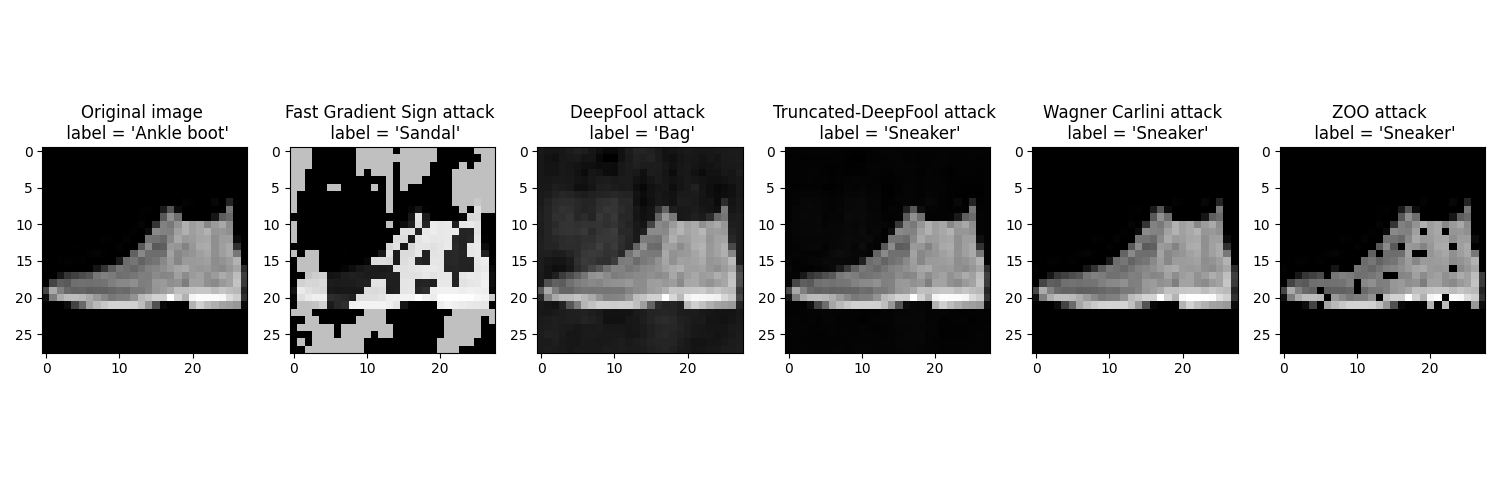
\includegraphics[width=\textwidth]{illustrations/attacks_sample_dfz.png}
    \caption{Comparison of different attacks on DFZ classifier}
    \label{fig:attacks_sample_dfz}
\end{figure*}

\begin{figure*}[ht]
    \centering
    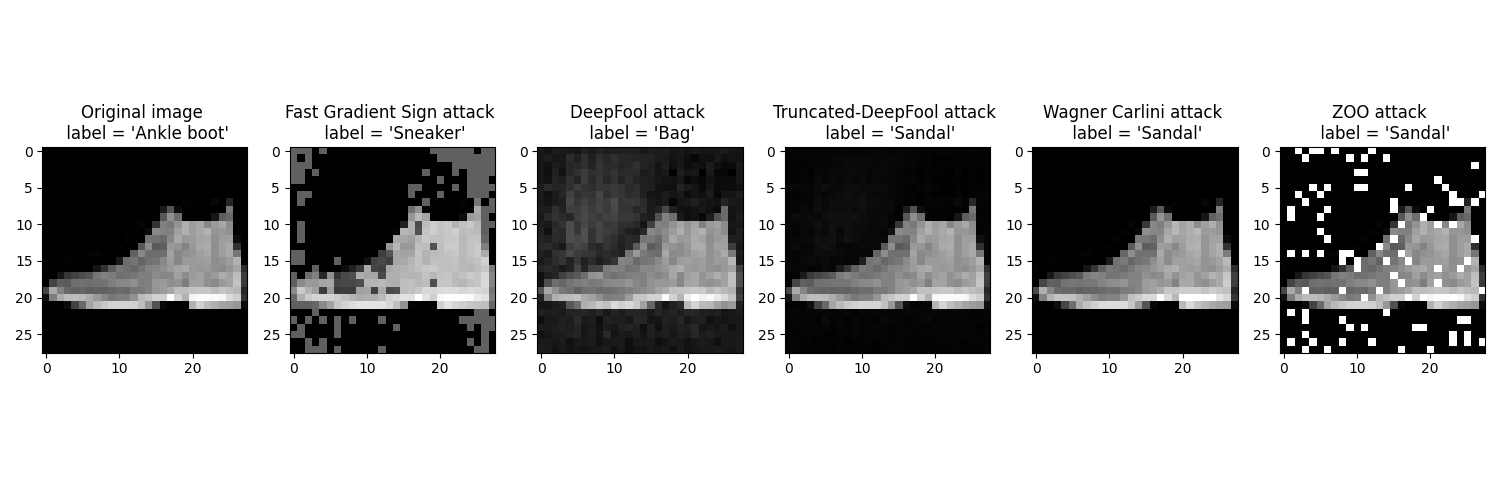
\includegraphics[width=\textwidth]{illustrations/attacks_sample_gfz.png}
    \caption{Comparison of different attacks on GFZ classifier}
    \label{fig:attacks_sample_gfz}
\end{figure*}

\begin{figure*}[ht]
    \centering
    \begin{minipage}[b]{0.49\textwidth}
        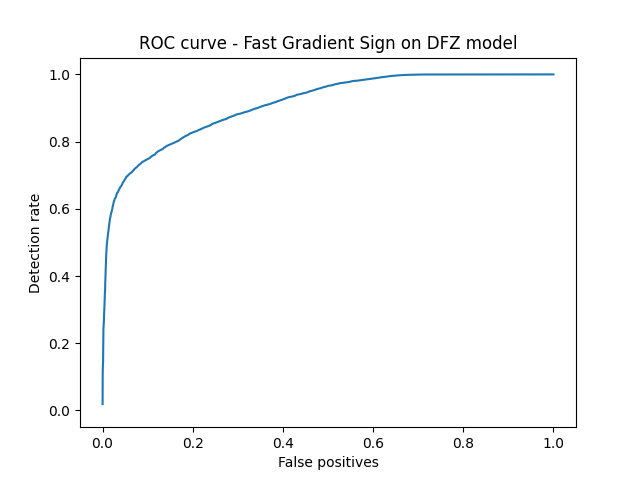
\includegraphics[width=\textwidth]{illustrations/ROC_Fast Gradient Sign_dfz.png}
        \caption{ROC curve for Fast Gradient Sign attack on DFZ}
        \label{fig:roc_fgs_dfz}
    \end{minipage}
    \hfill
    \begin{minipage}[b]{0.49\textwidth}
        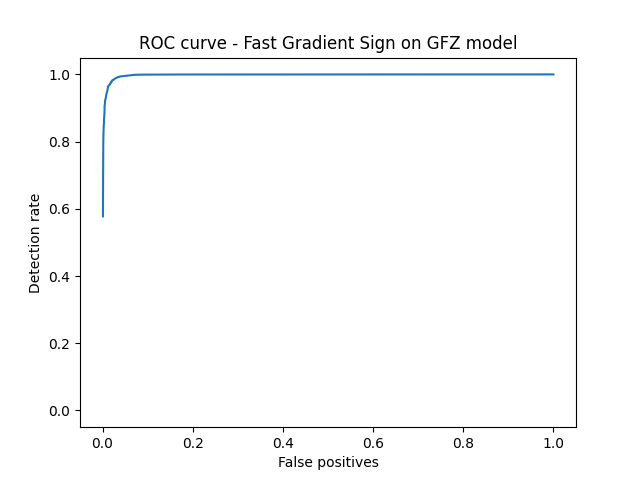
\includegraphics[width=\textwidth]{illustrations/ROC_Fast Gradient Sign_gfz.png}
        \caption{ROC curve for Fast Gradient Sign attack on GFZ}
        \label{fig:roc_fgs_gfz}
    \end{minipage}
\end{figure*}

\begin{figure*}[ht]
    \centering
    \begin{minipage}[b]{0.49\textwidth}
        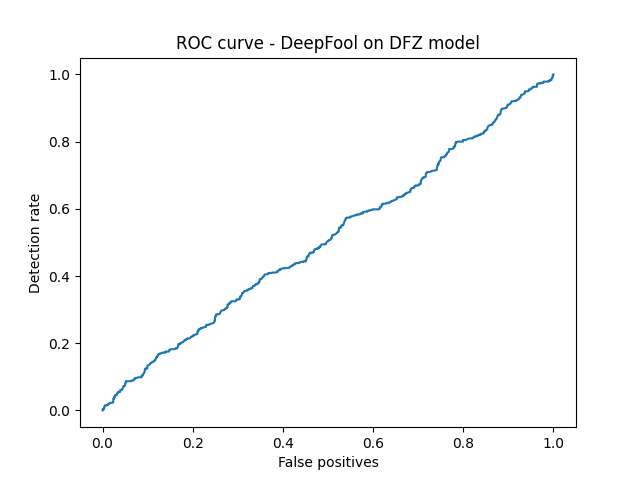
\includegraphics[width=\textwidth]{illustrations/ROC_DeepFool_dfz.png}
        \caption{ROC curve for DeepFool attack on DFZ}
        \label{fig:roc_deepfool_dfz}
    \end{minipage}
    \hfill
    \begin{minipage}[b]{0.49\textwidth}
        \includegraphics[width=\textwidth]{illustrations/ROC_DeepFool_gfz.png}
        \caption{ROC curve for DeepFool attack on GFZ}
        \label{fig:roc_deepfool_gfz}
    \end{minipage}
\end{figure*}

%%%%%%%%% REFERENCES
{\small
\bibliographystyle{acm}
\bibliography{biblio}
}

\end{document}
